\section{Multi Channel Routing protocol}
\label{MCRP}

\subsection{MCRP overview}
The goals of MCRP are (i) to reduce interference experienced through use of multiple channels and (ii) maximise the network lifetime by reconfiguring the topology. 
An initial version of Multichannel Cross-Layer Routing Protocol (MCRP) is introduced in~\cite{mcrp} but the version in this paper has extensive changes.  In particular this paper introduces the changes for energy based lifetime maximisation.

Multichannel Cross-Layer Routing Protocol (MCRP) \cite{mcrp} is a decentralised cross-layer protocol with a centralised controller based on RPL.  The system has two parts: a central algorithm which is typically run by the LPBR that allocated nodes to channels and assigns the topology; and a protocol which allows the network to communicate the channel change decision, probe the new channel and either communicate the success of the change or fall back to the previous channel. 

\subsection{Channel Selection Strategy}
\added{Without loss of generality, for the remainder of the paper we focus on the IEEE 802.15.4 MAC.} As in RPL, all nodes are initialised to channel 26 on start up and use the single channel RPL protocol to find initial neighbours.  Once the system is up and running a channel selection strategy is used based on information provided by MCRP about channel reliability.  Each node is assigned a listening channel.  Neighbours must send to the nodes on its listening channel.  The LPBR strategically selects the listening channels.  In this work we use a two-hop colouring algorithm inspired by the graph colouring problems~\cite{graphColouring}. The core idea is that no node should use the same listening channel as a neighbour or a neighbour of a neighbour (two hops).

In the two-hop colouring algorithm, the LPBR chooses a node $N$ to which it will assign a new channel $D$ to listen on.  MCRP chooses a random channel for $N$ for a potential swap according to the two-hop colouring rule that no node within two hops of $N$ is already coloured the same (listening on the same channel).  The channel switching protocol (described in the next section) will determine if the new channel has a better reception rate (lower interference) than the current channel.  The node selection algorithm iteratively changes one node channel at a time. 


\subsection{Channel Switching}
\label{sec:switching}

An attempt to change to a new channel (as described in the previous section) is communicated to node $N$.  The change itself is implemented by a distributed protocol and is initiated  by $N$. The change request will either result in the node changing to a new channel or reverting to its old channel and communicating this new state to its neighbours (and to the LPBR).  The full protocol is described in~\cite{mcrp}.  This paper introduces improvements to the protocol for measuring whether a change is desirable due to probing.

%Figure \ref{MCRP} shows the steps in the protocol.
%Upon receiving the channel change message, the node $N$ stores its current channel $C$ and communicates to all its neighbours the new channel $D$ that it wishes to change to. Those neighbours will update their neighbour tables to ensure that they now send to node $N$ on channel $D$.  The node $N$ begins the channel quality checking process with each neighbour in turn by sending them a probe request. If this process fails for any neighbour then the node reverts to channel $C$. Node $N$ informs its neighbours of the decision. The neighbours will update their neighbour table to transmit on channel $C$. If all channel quality checks succeed, the node $N$ will listens on channel $D$. Node $N$ does not send a confirmation message to the neighbours as it would be redundant since the neighbours already know the node $N$ listening channel. 

%\begin{figure}
%\centering
%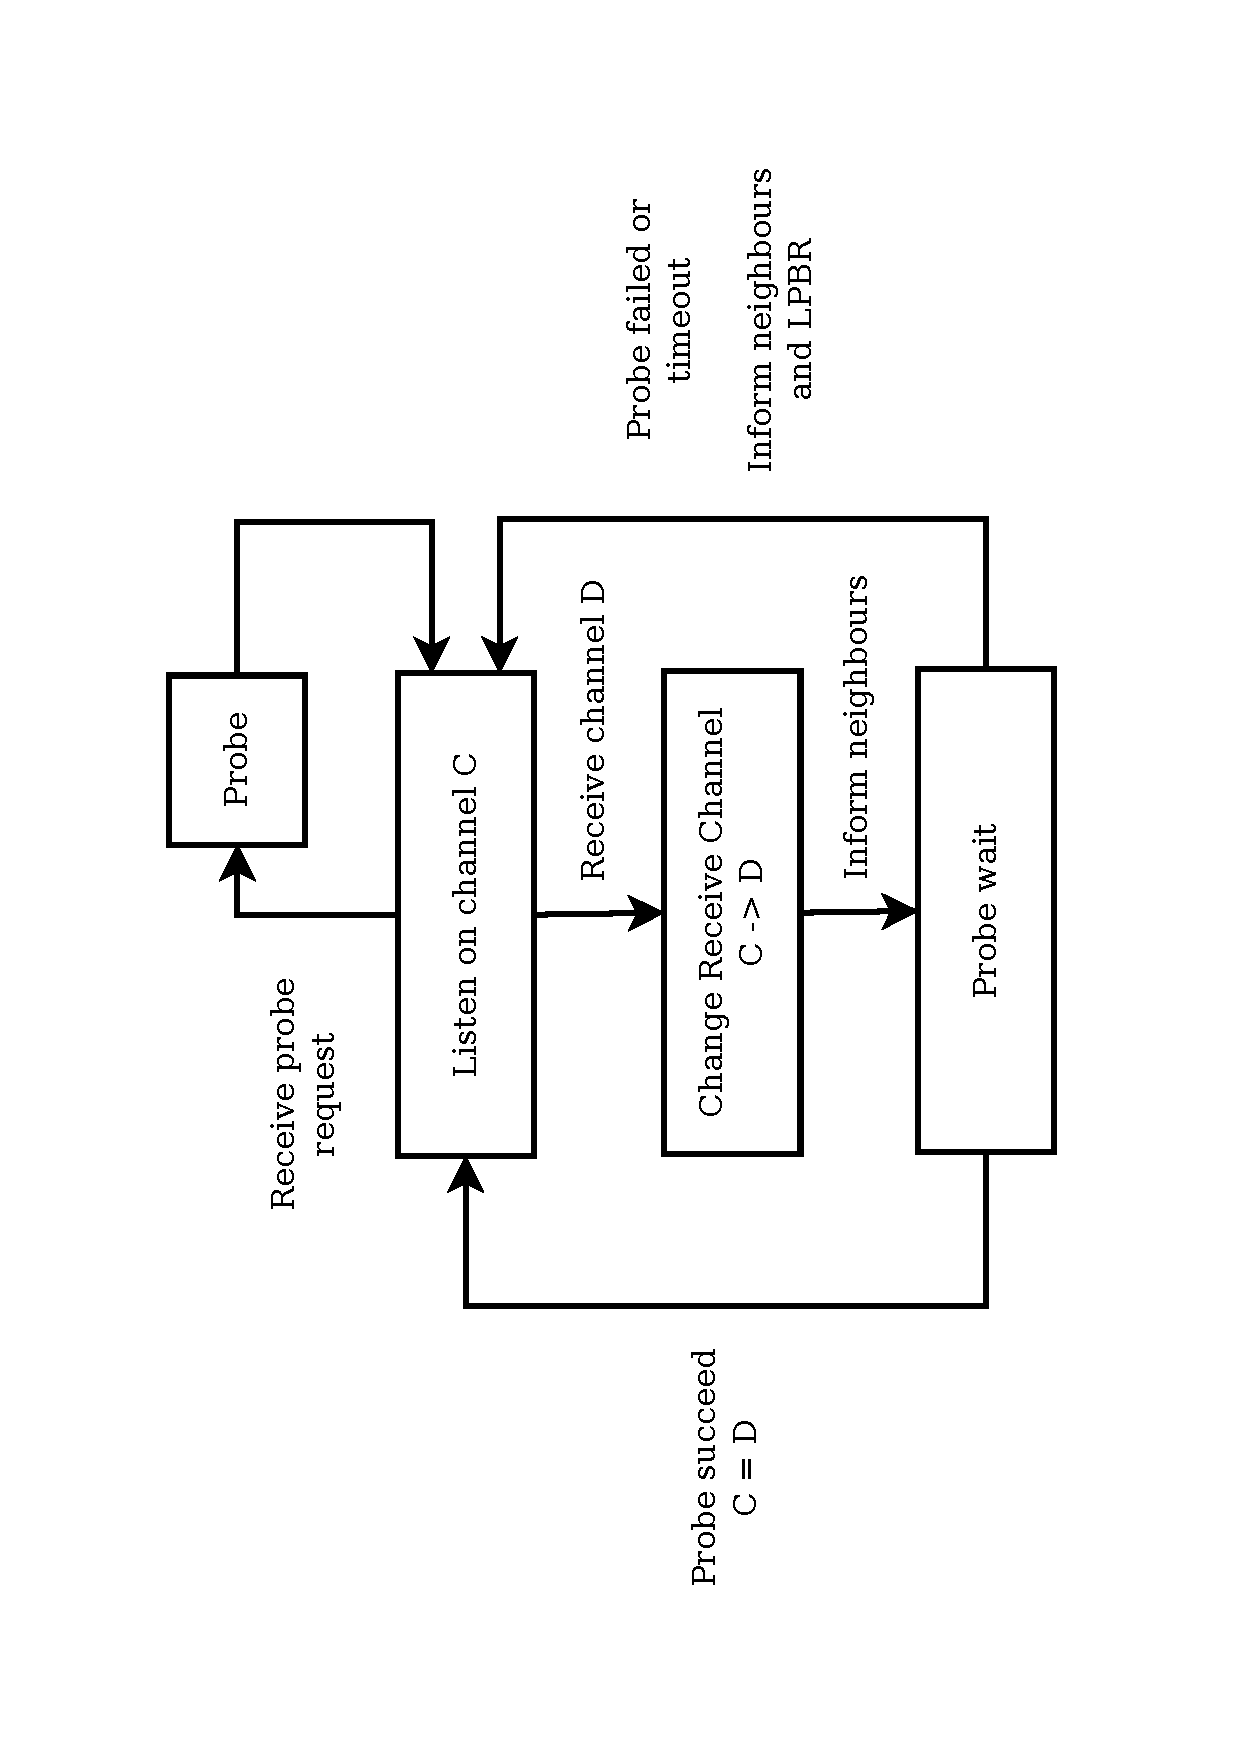
\includegraphics[trim=2cm 2cm 2cm 2cm, clip=true, totalheight=0.36\textheight, angle=270]{figures/channelSwitching.pdf}
%\caption{MCRP processes}
%\label{fig_mcrpDiagram}
%\end{figure}

Before a channel change MCRP uses probe packets between node $N$ and its neighbours to determine if the quality of channel is improved.  For each neighbour in turn eight probe packets are sent to $N$ on its new listening channel.  The number of packets received and the number of retransmissions required to receive them are monitored (in RPL several retransmissions are automatically tried).  The probing process fails if more than sixteen total transmissions are taken to receive eight packets on any link or if a timeout is reached before eight packets are received. In this case the node reverts to its previous channel.  The LPBR is informed of the results with a summary of all probes received and the channel so that the LPBR can build up a picture of channel strengths.

Because of the multichannel nature of MCRP a change is required to the RPL reconnection strategy to allow nodes that disconnect from their neighbour to find a new neighbour to connect to.  RPL uses a single channel and hence reconnection involves sending a message on this channel.  In MCRP these reconnection messages must be sent on multiple channels in turn as nodes are now listening on different channels.  New nodes and nodes which fall off the network can now rejoin on many potential channels.
